\section{Introduction}

Le but de ce draft est de présenter une proposition de découpage de la
solution proposée en réponse à l'appel d'offre de la COPEVUE.\\
Le système ébauché dans l'Ébauche de Conception Détaillée est découpé en
sous-système, puis en sous-projets. Cela est fait en vue de détailler
suffisamment le projet global pour en maîtriser la réalisation logicielle.

\subsection{Découpage en sous-systèmes}

\begin{figure}
\caption{Découpage en sous-systèmes}
\rotatebox{90}{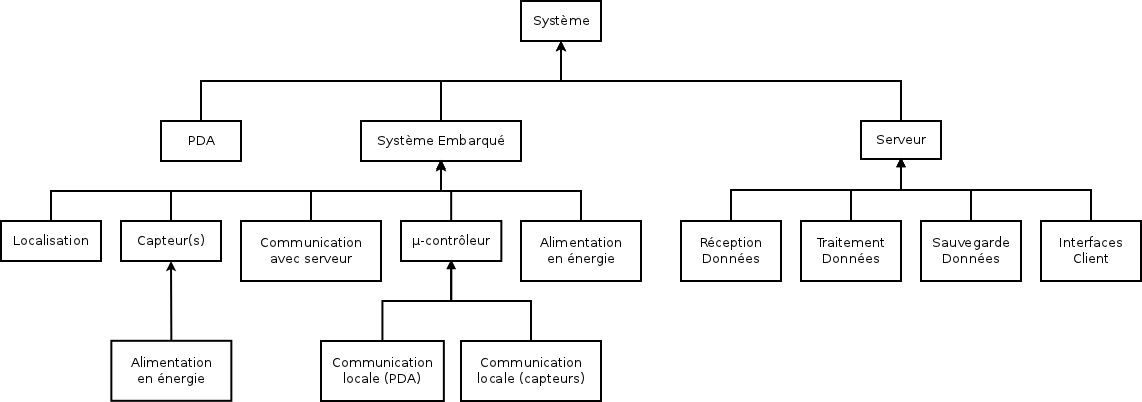
\includegraphics[scale=0.5]{\PIXPATH/decoupe1}}
\end{figure}

Ce diagramme présente le découpage en sous-sytème de notre solution, dont
on va tirer les sous-projets.

\subsection{Découpage en sous-projet}

Les sous-projets regroupent un ou plusieurs sous-systèmes selon les
critères suivants :
\begin{itemize}
\item fonctionnalité
\item transversalité
\item complexité
\end{itemize}

\hfill\\

On a donc les sous-projets suivants :
\begin{description}
\item[Installation et paramétrage de l'ERP]
\item[Conception matérielle du système embarqué]
\item[Programmation du système embarqué]
\item[Applicatif PDA]
\item[Intégration des différents sous-projets système]
\item[Documentation]
\item[Formation des futurs utilisateurs]
\end{description}
